% Part 2 — Stretch Problems

\begin{problem}[Dice probabilities and proportion thresholds]
\textit{A binomial/normal exercise on counts and proportions.}\\
Two fair dice are thrown repeatedly. In each throw, call the result a ``success'' if the sum of the two dice is at least $10$. Let $X$ count the number of successes in $n$ independent throws, and let $\hat p=X/n$ be the sample proportion of successes. This problem moves from the exact binomial model to the normal approximation, so be careful about when a continuity correction is being used.
\begin{enumerate}[label=\textbf{(\roman*)}]
\item Find the exact single-throw success probability $p$, then determine the minimum number of throws $n$ required so that $P(X\ge 2)>0{.}90$.

\item With $n=180$, approximate the probability that the number of successes is exactly equal to its expected value. Use a normal approximation to the binomial distribution with a continuity correction. You may use $\Phi(0{.}1)-\Phi(-0{.}1)\approx 0{.}0796$.

\item An observer wants the sample proportion $\hat p$ to fall within $0{.}05$ of the true probability $p$ with approximately $95\%$ probability. Ignoring continuity corrections, find the minimum suitable $n$. Use $\Phi^{-1}(0{.}975)\approx 1{.}96$.

\item Show algebraically that applying a continuity correction of $\pm 0{.}5$ to the count $X$ is equivalent to applying a correction of $\pm\frac{1}{2n}$ to the proportion $\hat p$.
\end{enumerate}

\begin{center}\small
\begin{tikzpicture}
  \begin{axis}[
      DLfigaxis,
      width=0.92\textwidth,
      height=3.6cm,
      xmin=18.5,
      xmax=41.5,
      ymin=0,
      ymax=0.12,
      enlargelimits=false,
      xlabel={success count (normal approx.\ $Y$)},
    ]
    \def\normy{exp(-((x-30)^2)/(2*25))/sqrt(2*pi*25)}

    \addplot[green!55!black, draw=none, fill=green!55!black, fill opacity=0.25, samples=220, smooth, domain=29.5:30.5]
      {\normy}\closedcycle;

    \addplot[green!45!black, thick, samples=240, smooth, domain=18.5:41.5]
      {\normy};

    \addplot[densely dashed, gray!75, mark=none, forget plot]
      coordinates {(29.5,0)(29.5,0.11)};
    \addplot[densely dashed, gray!75, mark=none, forget plot]
      coordinates {(30.5,0)(30.5,0.11)};

    \node[
      font=\scriptsize,
      align=left,
      fill=white,
      draw=gray!68,
      rounded corners=2pt,
      inner sep=4pt,
      anchor=north east,
      text width=4.95cm,
    ] at (axis cs:41, 0.115)
      {$\displaystyle P(\mu-\tfrac12\le Y\le\mu+\tfrac12)$\\[3pt]{\footnotesize continuity}};
  \end{axis}
\end{tikzpicture}\\[0.35em]

\noindent\footnotesize\textit{Dice problem ($n=180$, $\mu=30$, $\sigma=5$): ``exactly $30$ successes'' uses the continuity band $[29{.}5,30{.}5]$ on the approximating normal.}
\end{center}

\end{problem}

\begin{hint}
\begin{itemize}[leftmargin=*]
\item $P(X\ge 2)=1-P(0)-P(1)$; numerical search over $n$.
\item ``Exactly mean'' corresponds to interval $[\mu-\tfrac12,\,\mu+\tfrac12]$ for the approximating normal.
\item Margin $1{.}96\sqrt{p(1-p)/n}$.
\item Divide inequalities by $n$.
\end{itemize}
\end{hint}

\begin{solution}
\textbf{(i)} There are $36$ equally likely ordered outcomes. The sums at least $10$ are
$(4,6),(5,5),(6,4),(5,6),(6,5),(6,6)$, so
\[
p=\frac{6}{36}=\frac16,\qquad q=1-p=\frac56.
\]
For $X\sim B(n,\frac16)$,
\[
P(X\ge2)=1-P(X=0)-P(X=1).
\]
Thus we need
\[
\left(\frac56\right)^n+n\left(\frac16\right)\left(\frac56\right)^{n-1}<0{.}10.
\]
Testing integer values gives $n=21$ too small, while $n=22$ works, so the minimum is $\boxed{22}$ throws.

\textbf{(ii)} When $n=180$, the binomial mean and variance are
\[
\mu=np=30,\qquad \sigma^2=npq=180\cdot\frac16\cdot\frac56=25.
\]
Exactly $30$ successes is represented by the continuous interval $29{.}5\le Y\le30{.}5$, where $Y\sim N(30,25)$. Hence
\[
z_1=\frac{29{.}5-30}{5}=-0{.}1,\qquad
z_2=\frac{30{.}5-30}{5}=0{.}1,
\]
so the required probability is approximately
\[
P(-0{.}1\le Z\le0{.}1)=\Phi(0{.}1)-\Phi(-0{.}1)\approx \boxed{0{.}0796}.
\]

\textbf{(iii)} The approximate standard deviation of $\hat p$ is
\[
\sqrt{\frac{p(1-p)}{n}}=\sqrt{\frac{5}{36n}}.
\]
For a central $95\%$ interval, require
\[
1{.}96\sqrt{\frac{5}{36n}}\le0{.}05.
\]
Squaring and rearranging gives $n\ge213{.}42\ldots$, so the minimum integer is $\boxed{214}$.

\textbf{(iv)} Since $\hat p=X/n$ and $n>0$, dividing the count inequality by $n$ preserves the inequality directions:
\[
x-\frac12\le X\le x+\frac12
\quad\Longleftrightarrow\quad
\frac{x}{n}-\frac{1}{2n}\le \frac{X}{n}\le \frac{x}{n}+\frac{1}{2n}.
\]
Therefore
\[
\frac{x}{n}-\frac{1}{2n}\le \hat p\le \frac{x}{n}+\frac{1}{2n}.
\]
\end{solution}

\begin{takeaways}
\item A binomial model begins with one clear success probability.
\item Continuity correction turns a single count into a width-one interval.
\item On the proportion scale, the correction shrinks from $\pm0{.}5$ to $\pm\frac{1}{2n}$.
\end{takeaways}

\begin{problem}[Simulating a binomial by coin tosses (enrichment)]
\textit{Enrichment: uses short Python; not examinable as a fixed-item in HSC.}

Simulate $B(10,\tfrac12)$ as the count of heads in ten fair coin flips. One simulated experiment consists of ten flips; the recorded value is the number of heads. By repeating that experiment many times, you can see the empirical histogram cluster around the theoretical mean $np=5$.

\begin{verbatim}

    import random
    N = 20000 # number of simulated experiments
    results = []
    for _ in range(N):
        heads = sum(random.random() < 0.5 for _ in range(10))
        results.append(heads)
    # Optional: print mean and rough histogram
    from collections import Counter
    c = Counter(results)
    print("mean count", sum(results)/N)
    print("counts", dict(sorted(c.items())))

\end{verbatim}

% \begin{verbatim}
% import random
% N = 20000            # number of simulated experiments
% results = []
% for _ in range(N):
%     heads = sum(random.random() < 0.5 for _ in range(10))
%     results.append(heads)

% # Optional: print mean and rough histogram
% from collections import Counter
% c = Counter(results)
% print("mean count", sum(results)/N)
% print("counts", dict(sorted(c.items())))
% \end{verbatim}

\textbf{Task.} Run the script, for example in Google Colab. Report the sample mean and comment on how close it is to $np=5$. Explain why increasing $N$, the number of simulated experiments, sharpens the agreement between simulation and theory.
\end{problem}

\begin{hint}
\begin{itemize}[leftmargin=*]
\item Each experiment is independent; mean of counts estimates $np$.
\item Law of Large Numbers reduces Monte Carlo noise.
\end{itemize}
\end{hint}

\begin{solution}
Each simulated experiment has expected count
\[
E(X)=np=10\cdot\frac12=5.
\]
Your printed sample mean will not usually equal $5$ exactly, because the simulation itself is random. However, it should be close to $5$ when $N=20000$. If $N$ is increased, the average is taken over more independent experiments, so the random simulation error tends to shrink. This is a computational version of the Law of Large Numbers.


Expected result: 

\begin{verbatim}

    mean count 5.00115
    counts {0: 16, 1: 184, 2: 879, 3: 2339, 4: 4055, 
            5: 4997, 6: 4128, 7: 2322, 
            8: 900, 9: 163, 10: 17}

\end{verbatim}

\end{solution}

\begin{takeaways}
\item A binomial random variable can be simulated by repeating Bernoulli trials and counting successes.
\item Simulation output is random, so exact agreement is not expected.
\item Larger Monte Carlo sample sizes give more stable estimates.
\end{takeaways}

\begin{problem}[Calculating normal probabilities with Python (enrichment)]
\textit{Enrichment laboratory; software skills are illustrative.}

Assume IQ scores in a population are modelled by $X\sim N(100,15^{2})$. The value $115$ is one standard deviation above the mean. Use Python to compute the left-tail probability $P(X\le115)$, and compare the result with the standard normal table value $\Phi(1)$.

\begin{verbatim}
    from scipy.stats import norm
    print(norm.cdf(115, loc=100, scale=15))
\end{verbatim}

Compare the output to $\Phi(1)=0{.}8413$.
\end{problem}

\begin{hint}
\begin{itemize}[leftmargin=*]
\item SciPy \texttt{norm.cdf} applies the cdf with explicit mean/scale arguments.
\item $z=(115-100)/15=1$.
\end{itemize}
\end{hint}

\begin{solution}
Standardising gives
\[
z=\frac{115-100}{15}=1.
\]
Therefore
\[
P(X\le115)=P(Z\le1)=\Phi(1)\approx0{.}8413.
\]
The Python command \texttt{norm.cdf(115, loc=100, scale=15)} applies the same calculation directly using the original mean and standard deviation, so it should print approximately $0{.}8413$.


Expected result: 

\begin{verbatim}
    0.8413447460685429
\end{verbatim}

\end{solution}

\begin{takeaways}
\item Software cdf commands and standard normal tables are evaluating the same probability.
\item The \texttt{loc} parameter is the mean; the \texttt{scale} parameter is the standard deviation.
\item Standardising first is still useful for checking whether the output is reasonable.
\end{takeaways}

\begin{problem}[Rare blue variants and sample proportions]
In a breeding experiment, the true long-run proportion of blue offspring is believed to be $p=0{.}20$. Let $\hat p$ denote the observed sample proportion. Because the sample sizes in this problem are large, we will approximate the distribution of $\hat p$ using a normal distribution.

\textbf{(i)}\ For $n=500$, approximate the probability that strictly more than $22\%$ of the flowers are blue. Use a continuity correction by translating ``strictly more than $110$ blue flowers'' to the boundary $110{.}5$.

\textbf{(ii)}\ Find the smallest integer $n$ for which the normal approximation gives
\[
P(|\hat p-p|<0{.}03)\ge0{.}99.
\]
\begin{center}\small
\begin{tikzpicture}
  \begin{axis}[
      DLfigaxis,
      width=0.9\textwidth,
      height=2.95cm,
      xmin=0.145,
      xmax=0.268,
      ymin=0,
      ymax=24,
      xlabel={sample proportion $\hat p$},
      clip=false,
    ]
    \def\phhat{0.20}
    \addplot[red!78!black, draw=none, fill=red!78!black, fill opacity=0.18,
      samples=180, smooth, domain=0.221:0.265]
      {exp(-((x-\phhat)^2)/(2*(0.00032)))/sqrt(2*pi*(0.00032))};

    \addplot[red!62!black, thick,
      samples=220, smooth, domain=0.145:0.265]
      {exp(-((x-\phhat)^2)/(2*(0.00032)))/sqrt(2*pi*(0.00032))};

    \addplot+[const plot, densely dashed, gray!78, forget plot]
      coordinates {(0.2002,24)(0.2002,0)};
    \addplot+[const plot, densely dashed, gray!78, forget plot]
      coordinates {(0.221,24)(0.221,0)};

  \end{axis}
\end{tikzpicture}\\[0.3em]

\noindent\footnotesize\textit{$p=0{.}20$ versus continuity boundary $110{.}5/500=0{.}221$ (shaded right tail). Uses $\mathrm{Var}(\hat p)\approx pq/n$ with $p=0{.}2$, $n=500$.}
\end{center}

\end{problem}

\begin{hint}
\begin{itemize}[leftmargin=*]
\item Carry counts to proportion scale before evaluating $z$ on proportions.
\item For (ii), set $z_{0{.}995}\approx 2{.}576$ (or cite your table) $\times\sqrt{pq/n}$.
\end{itemize}
\end{hint}

\begin{solution}
\textbf{(i)} For the sample proportion,
\[
\mu_{\hat p}=p=0{.}20,\qquad
\sigma_{\hat p}=\sqrt{\frac{pq}{n}}=\sqrt{\frac{0{.}2\cdot0{.}8}{500}}.
\]
Strictly more than $22\%$ means more than $110$ blue flowers out of $500$, so the continuity-corrected boundary is
\[
\hat p>\frac{110{.}5}{500}=0{.}221.
\]
Thus
\[
z=\frac{0{.}221-0{.}20}{\sqrt{0{.}16/500}}\approx1{.}17.
\]
The probability is approximately
\[
P(Z>1{.}17)=1-\Phi(1{.}17)\approx \boxed{0{.}12}.
\]

\textbf{(ii)} A central $99\%$ normal interval uses $z_{0{.}995}\approx2{.}576$. We need the margin of error to be at most $0{.}03$:
\[
2{.}576\sqrt{\frac{0{.}2\cdot0{.}8}{n}}\le0{.}03.
\]
Rearranging,
\[
n\ge\left(\frac{2{.}576\sqrt{0{.}16}}{0{.}03}\right)^2\approx1179{.}9.
\]
Since $n$ must be an integer, the minimum is $\boxed{1180}$ seeds.
\end{solution}

\begin{takeaways}
\item For sample proportions, use mean $p$ and standard deviation $\sqrt{pq/n}$.
\item A count-based continuity correction can be converted to a proportion boundary.
\item High confidence and a small margin of error require a large sample size.
\end{takeaways}

\begin{problem}[Advanced inheritance scenarios]
A horticulturalist is attempting to cross two species of flowers to isolate a rare ``true crimson'' colour variant. According to the genetic model, each offspring independently has probability $0{.}25$ of displaying the true crimson colour. For a large planting of $400$ offspring, let $C\sim B(400,0{.}25)$ count the number of crimson flowers. In part (i), use a smaller greenhouse count $X\sim B(20,0{.}25)$.
\begin{enumerate}[label=\textbf{(\roman*)}]
\item In the greenhouse of $20$ offspring, find the conditional probability that exactly $5$ flowers are true crimson, given that at least one flower is true crimson.
\item Determine the minimum number of offspring $n$ that must be cultivated to ensure at least a $99\%$ probability of obtaining two or more true crimson flowers.
\item For the commercial planting of $400$ offspring, approximate $P(90\le C\le110)$ using a normal approximation with continuity correction.
\item A competing scientist tests a soil additive on $400$ plants and observes $120$ true crimson flowers. Find the uncorrected $z$-score relative to the baseline $p=0{.}25$, and briefly comment on the evidence.
\end{enumerate}

\begin{center}\small
\begin{tikzpicture}
  \begin{axis}[
      DLfigaxis,
      width=0.92\textwidth,
      height=3.65cm,
      xmin=78,
      xmax=123,
      ymin=0,
      ymax=0.062,
      enlargelimits=false,
      xlabel={crimson count $C$ (normal approx.)},
    ]
    \def\nc{exp(-((x-100)^2)/(2*75))/sqrt(2*pi*75)}

    \addplot[cyan!55!black, draw=none, fill=cyan!55!black, fill opacity=0.22, samples=280, smooth, domain=89.5:110.5]
      {\nc}\closedcycle;

    \addplot[cyan!45!black, thick, samples=360, smooth, domain=78:123]
      {\nc};

    \addplot[densely dashed, gray!78, mark=none, forget plot]
      coordinates {(89.5,0)(89.5,0.06)};
    \addplot[densely dashed, gray!78, mark=none, forget plot]
      coordinates {(110.5,0)(110.5,0.06)};

    \node[
      font=\scriptsize,
      align=left,
      fill=white,
      draw=gray!68,
      rounded corners=2pt,
      inner sep=4pt,
      anchor=north east,
      text width=6.9cm,
    ] at (axis cs:122, 0.059)
      {$P(90\le C\le110)$\\[3pt]{\footnotesize$\displaystyle \approx P(89{.}5\le Y\le110{.}5)$}};
  \end{axis}
\end{tikzpicture}\\[0.35em]

\noindent\footnotesize\textit{Inheritance (iii): inclusive binomial counts $90$--$110$ become the continuity window $[89{.}5,110{.}5]$ on $N(100,75)$.}
\end{center}

\end{problem}

\begin{hint}
\begin{itemize}[leftmargin=*]
\item Conditional formula; complement for tail $1-P(0)-P(1)$.
\item Normal parameters $\mu=np$, $\sigma=\sqrt{npq}$.
\item Two-sided continuity ($89{.}5,\,110{.}5$).
\end{itemize}
\end{hint}

\begin{solution}
\textbf{(i)} Let $X\sim B(20,0{.}25)$ for the greenhouse. Since the event $X=5$ automatically implies $X\ge1$,
\[
P(X=5\mid X\ge1)=\frac{P(X=5)}{P(X\ge1)}.
\]
Now
\[
P(X=5)=\binom{20}{5}(0{.}25)^5(0{.}75)^{15}\approx0{.}2023,
\]
and
\[
P(X\ge1)=1-P(X=0)=1-0{.}75^{20}\approx0{.}9968.
\]
Therefore
\[
P(X=5\mid X\ge1)\approx\frac{0{.}2023}{0{.}9968}\approx \boxed{0{.}2030}.
\]

\textbf{(ii)} Let $C_n\sim B(n,0{.}25)$. The complement of ``two or more'' is ``zero or one'', so
\[
P(C_n\ge2)=1-P(C_n=0)-P(C_n=1).
\]
We need
\[
0{.}75^n+n(0{.}25)(0{.}75)^{n-1}\le0{.}01.
\]
Factoring gives
\[
0{.}75^{n-1}(0{.}75+0{.}25n)\le0{.}01.
\]
Testing nearby integers, $n=23$ gives approximately $0{.}0116$, which is still too large. For $n=24$, the value is approximately $0{.}0090$, so the minimum is $\boxed{24}$ offspring.

\textbf{(iii)} For $C\sim B(400,0{.}25)$,
\[
\mu=np=100,\qquad \sigma=\sqrt{npq}=\sqrt{400(0{.}25)(0{.}75)}=\sqrt{75}.
\]
The inclusive event $90\le C\le110$ becomes
\[
89{.}5\le Y\le110{.}5,\qquad Y\sim N(100,75).
\]
The $z$-values are
\[
z_1=\frac{89{.}5-100}{\sqrt{75}}\approx-1{.}21,\qquad
z_2=\frac{110{.}5-100}{\sqrt{75}}\approx1{.}21.
\]
Hence
\[
P(90\le C\le110)\approx P(-1{.}21\le Z\le1{.}21)\approx \boxed{0{.}774}.
\]

\textbf{(iv)} Under the baseline model, $120$ crimson flowers is compared with mean $100$ and standard deviation $\sqrt{75}$. The uncorrected score is
\[
z=\frac{120-100}{\sqrt{75}}\approx \boxed{2{.}31}.
\]
This is more than two standard deviations above the baseline mean, so it would be considered unusually high under the $25\%$ model and gives strong evidence that the additive may have increased the crimson rate.
\end{solution}

\begin{takeaways}
\item Conditioning removes part of the sample space; here it removes only the zero-crimson case.
\item Minimum sample-size questions often use the complement and then test integers.
\item Continuity corrections are essential when a normal curve approximates inclusive binomial counts.
\end{takeaways}

\begin{problem}[Memoryless geometric distribution]
Suppose independent trials are repeated until the first success occurs. Let $X$ be the waiting time, counted as the trial number of the first success. If the success probability on each trial is $p$ and $q=1-p$, then
\[
P(X=x)=pq^{x-1},\qquad x=1,2,\ldots
\]
Assume $E[X]=1/p$.
\begin{enumerate}[label=\textbf{(\roman*)}]
\item Show $P(X>n)=q^{n}$.
\item Prove $P(X>n+k\mid X>n)=P(X>k)$, and briefly explain why this is called the memoryless property.
\item By differentiating the geometric series twice, show $\mathrm{Var}(X)=q/p^{2}$.
\item A space probe attempts to ping a satellite every $4$ seconds. Each ping succeeds with probability $0{.}05$. Find the mean and standard deviation of the total waiting time $T=4X$ seconds.
\end{enumerate}

\begin{center}\small
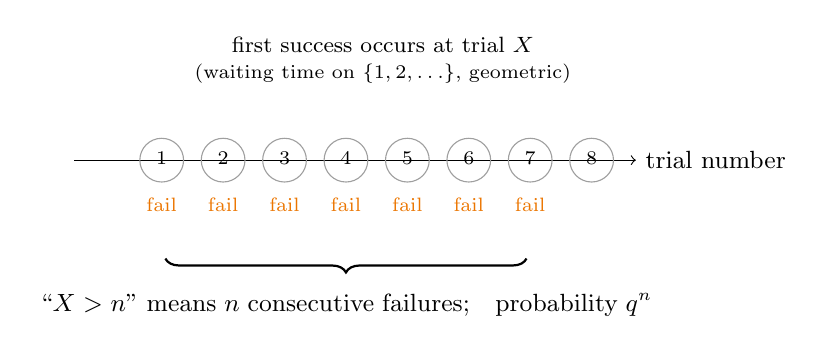
\begin{tikzpicture}[x=0.78cm,y=1cm]

  % Explain the picture above the numbered trials (nothing overlaps circles or ``fail'' row)
  \node[
    align=center,
    font=\footnotesize,
  ] at (4.6, 1.62)
    {first success occurs at trial $X$\\
     {\scriptsize (waiting time on $\{1,2,\ldots\}$, geometric)}};

  \draw[->] (-0.42, 0.35) -- (8.72, 0.35)
    node[right, font=\small] {trial number};

  % Trial markers — row $y = 0.35$
  \foreach \t in {1,...,8}{
    \node[
      circle,
      draw=gray!75,
      minimum size=1.58em,
      inner sep=0pt,
      font=\scriptsize,
    ] at (\t, 0.35) {\strut$\t$};
  }

  % Outcomes row: one ``fail'' word per column (trials $1$--$7$)
  \foreach \t in {1,...,7}{
    \node[
      anchor=north,
      font=\scriptsize,
      text=orange!92!black,
    ] at (\t, 0.02) {\strut fail};
  }

  % Brace spanning trials $1,\ldots,n$ illustrating $q^n$
  \draw[thick, decorate, decoration={brace, mirror, amplitude=5pt}]
    (1.06, -0.90) -- (6.94, -0.90)
    node[
      midway,
      below=9pt,
      font=\footnotesize,
      align=center,
      text width=7.85cm,
    ]
    {\small ``$X>n$'' means $n$ consecutive failures;\quad probability $q^n$};

\end{tikzpicture}\\[2.55em]

\noindent\footnotesize\textit{Geometric waiting picture: memorylessness compares $P(X>n+k\mid X>n)$ with fresh starts.}
\end{center}

\end{problem}

\begin{hint}
\begin{itemize}[leftmargin=*]
\item Intersection $X>n{+}k$ inside $X>n$ is just the former event.
\item Differentiate $\sum q^{x}$ or use known factorial moment route.
\item $\mathrm{Var}(4X)=16\mathrm{Var}(X)$.
\end{itemize}
\end{hint}

\begin{solution}
\textbf{(i)} The event $X>n$ means the first $n$ trials all fail. Since the trials are independent, this has probability $q^n$. Equivalently,
\[
P(X>n)=\sum_{x=n+1}^{\infty}pq^{x-1}
=pq^n(1+q+q^2+\cdots)=\frac{pq^n}{1-q}=q^n.
\]

\textbf{(ii)} Using conditional probability,
\[
P(X>n+k\mid X>n)=\frac{P(X>n+k)}{P(X>n)}
=\frac{q^{n+k}}{q^n}=q^k.
\]
But $q^k=P(X>k)$. This says that, after $n$ failures, the probability of needing more than $k$ additional trials is the same as it was at the start.

\textbf{(iii)} From
\[
\sum_{x=0}^{\infty}q^x=\frac{1}{1-q},
\]
differentiating twice gives
\[
\sum_{x=2}^{\infty}x(x-1)q^{x-2}=\frac{2}{(1-q)^3}.
\]
Multiplying by $pq$ gives
\[
E[X(X-1)]=\sum_{x=1}^{\infty}x(x-1)pq^{x-1}=\frac{2q}{p^2}.
\]
Then
\[
E[X^2]=E[X(X-1)]+E[X]=\frac{2q}{p^2}+\frac1p,
\]
so
\[
\mathrm{Var}(X)=E[X^2]-[E(X)]^2=\frac{q}{p^2}.
\]

\textbf{(iv)} Here $p=0{.}05$ and $q=0{.}95$. Thus
\[
E(X)=\frac1{0{.}05}=20,\qquad
\mathrm{Var}(X)=\frac{0{.}95}{0{.}05^2}=380.
\]
Since $T=4X$,
\[
E(T)=4E(X)=80\text{ s},\qquad
\mathrm{SD}(T)=4\sqrt{380}\approx \boxed{78\text{ s}}.
\]
\end{solution}

\begin{takeaways}
\item A geometric tail can be read as ``all previous trials failed.''
\item Memorylessness means past failures do not change the future waiting-time distribution.
\item Scaling time by $4$ scales the standard deviation by $4$ as well.
\end{takeaways}
